
%%%%%%%%%%%%%%%%%%%%%%% file typeinst.tex %%%%%%%%%%%%%%%%%%%%%%%%%
%
% This is the LaTeX source for the instructions to authors using
% the LaTeX document class 'llncs.cls' for contributions to
% the Lecture Notes in Computer Sciences series.
% http://www.springer.com/lncs       Springer Heidelberg 2006/05/04
%
% It may be used as a template for your own input - copy it
% to a new file with a new name and use it as the basis
% for your article.
%
% NB: the document class 'llncs' has its own and detailed documentation, see
% ftp://ftp.springer.de/data/pubftp/pub/tex/latex/llncs/latex2e/llncsdoc.pdf
%
%%%%%%%%%%%%%%%%%%%%%%%%%%%%%%%%%%%%%%%%%%%%%%%%%%%%%%%%%%%%%%%%%%%


\documentclass[runningheads,a4paper]{llncs}

\usepackage{amssymb}
\setcounter{tocdepth}{3}
\usepackage{graphicx}
\usepackage{multirow}
\usepackage[table,xcdraw]{xcolor}
\usepackage{algorithm}
\usepackage{algorithmic}
\usepackage{amsmath}
\usepackage{natbib}
\usepackage{graphicx} 
\usepackage{subfigure}
\usepackage{empheq}


\usepackage{url}
\urldef{\mailsa}\path|{alfred.hofmann, ursula.barth, ingrid.haas, frank.holzwarth,|
\urldef{\mailsb}\path|anna.kramer, leonie.kunz, christine.reiss, nicole.sator,|
\urldef{\mailsc}\path|erika.siebert-cole, peter.strasser, lncs}@springer.com|
\newcommand{\keywords}[1]{\par\addvspace\baselineskip
\noindent\keywordname\enspace\ignorespaces#1}

\begin{document}

\mainmatter  % start of an individual contribution

% first the title is needed
\title{A general framework \\for evaluating interactive 
image segmentation algorithms}

% a short form should be given in case it is too long for the running head
\titlerunning{A general framework for evaluating interactive 
segmentation algorithms}

% the name(s) of the author(s) follow(s) next
%
% NB: Chinese authors should write their first names(s) in front of
% their surnames. This ensures that the names appear correctly in
% the running heads and the author index.
%
\author{Bingjie Jiang%
\thanks{Please note that the LNCS Editorial assumes that all authors have used
the western naming convention, with given names preceding surnames. This determines
the structure of the names in the running heads and the author index.}%
\and Tonwei Ren}
%
% (feature abused for this document to repeat the title also on left hand pages)

% the affiliations are given next; don't give your e-mail address
% unless you accept that it will be published
\institute{Springer-Verlag, Computer Science Editorial,\\
Tiergartenstr. 17, 69121 Heidelberg, Germany\\
\mailsa\\
\mailsb\\
\mailsc\\
\url{http://www.springer.com/lncs}}



\toctitle{Lecture Notes in Computer Science}
\tocauthor{Authors' Instructions}
\maketitle


\begin{abstract}
The abstract should summarize the contents of the paper and should
contain at least 70 and at most 150 words. It should be written using the
\emph{abstract} environment.
\keywords{We would like to encourage you to list your keywords within
the abstract section}
\end{abstract}


\section{Introduction}
  \paragraph{}Interactive image segmentation has been extensively studied in the latest decade. Many state-of-the-art algorithms in this field have been proposed, starting from Boycov et. al\citep{boykov2001interactive},followed by Grabcut\citep{rother2004grabcut},Random Walker\citep{grady2006random},Bai and Sapiro \citep{bai2007geodesic} and \citep{gulshan2010geodesic}. However, when it comes to the evaluation of these algorithms, the comparison can hardly be objective due to different human interferences. As is often the case, interactive image segmentation algorithms are tested upon user scribbles provided by the specific author. In this way, the performance of segmentation result could heavily depend on certain batch of seeds selection, rendering the result not convincing enough when compared with other algorithms. 
 \paragraph{}This paper deals with the problem of evaluating interactive segmentation algorithms in an objective and comprehensive way. The contribution of this paper includes: (1)  Analysis of differences between user labels in a quantitative way. By clustering colors in the image, we figured out the correspondence between user labels and color clusters. 
 (2)...
 \paragraph{} The remainder of this paper is organized as follows:...
  
\section{Related Work}

******

\section{User-interaction differences}

\subsection{Dataset design}
\paragraph{}The dataset contains 96 images from publicly available Berkeley Segmentation Dataset\citep{martin2001database}. These images are selected so that each of them contains at least one obvious object which could be unambiguously explained to participants.These images are representative of some major challenges of image segmentation, including fuzzy boundary, complex texture and complex lighting conditions. Ground truths are precisely hand-labeled for each image in order to avoid any bias.


\subsection{Experiment}
\paragraph{}In this section we will discuss the design of experiment. We use the software provided by The K-Space Segmentation Tool Set, \citep{mcguinness2008k}. Screenshots of the tool are shown in Figure  \ref{fig:screenshot}. The 5 participants are all students from computer science background but have limited knowledge in interactive image segmentation. Each participant was given a clear guidance and enough time to familiarize themselves and become proficient with the software that would be used for the experiment. Sample markers were also provided in avoid of misunderstanding . Then in real experiment, each participants are provided with 96 images and the corresponding ground-truth which tells exactly which object to extract. However, we hide the segmentation result from user so that they will not realize if they have provided a "good" mark or not. We also confined the time for labeling each image. In this way, we manage to (1)limit the effort of participants to draw scribbles in consideration of real-life application.(2)obtain the most natural response of users rather than inputs guided by segmentation result.
\begin{figure}[h!]
\centering
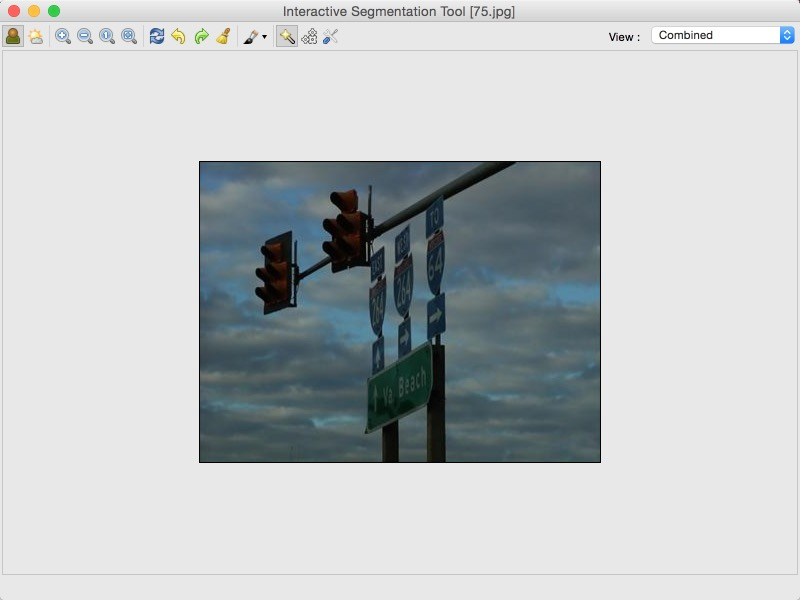
\includegraphics[width=0.5\columnwidth]{images/screenshot.png}
\textbf{\caption{ The screenshot of k-space segmentation tool}}
\label{fig:screenshot}
\end{figure}

\subsection{User-interaction differences}
 \paragraph{}In our person-oriented experiments, great differences among user labels were observed. It comes to us instinctively that different people tend to consider different part of foreground and background object as salient. Under this guidance, we processed the 5 marker files of each image out of the dataset and calculated the pair-wise intersection degree. The result is shown in table \ref{ta:intersection degree f}and table \ref{ta:intersection degree b}. The intersection degree is defined as follows:
$$intersection\ of\ marked\ pixels/union\ of\ marked\ pixels$$

\paragraph{}Table \ref{ta:intersection degree f} visualizes the value on foreground and Table \ref{ta:intersection degree b} the background. We make the following observations: (1)The average value of intersection/union between two people is rather low, ranging from 1.6592\% to 3.5195\% in foreground and 0.0905\% to 0.9700\% in background, which indicates that markers of different people have little common in common.Figure \ref{fig:example} shows an example of user markers which share no common pixel (2) People share less similarities in background markers than foreground. It is because the foreground objects are confined to a certain area while the backgrounds are more extensive. 


\begin{table}
\centering
\begin{tabular}{|c|c|c|c|c|c|}
\hline
 & seed 1 & seed 2 & seed 3 & seed 4& seed 5 \\
\hline
seed 1 & 100\% & 2.3768\% & 3.5195\% & 2.0146\%& 1.6592\% \\
\hline
seed 2 & 2.3768\% & 100\% & 2.7080\% & 2.1684\%& 2.2459\% \\
\hline
seed 3 & 3.5195\% & 2.7080\% & 100\% & 2.0485\%& 2.0102\%\\
\hline
seed 4 & 2.0146\% & 2.1684\% & 2.0485\% & 100\%& 1.8441\% \\
\hline
seed 5 & 1.6592\% & 2.2459\% & 2.0102\% & 1.8441\%& 100\% \\
\hline
\end{tabular}
\caption{intersection degree of foreground}
\label{ta:intersection degree f}
\end{table} 

\begin{table}
\centering
\begin{tabular}{|c|c|c|c|c|c|}
\hline
 Seed & seed 1 & seed 2 & seed 3 & seed 4& seed 5 \\
\hline
seed 1 & 100\% & 0.8700\% & 0.8600\% & 0.0905\%& 0.6300\% \\
\hline
seed 2 & 0.8700\% & 100\% & 0.9700\% & 0.2100\%& 0.7300\% \\
\hline
seed 3 & 0.8600\% & 0.9700\% & 100\% & 0.1600\%& 0.6800\%\\
\hline
seed 4 & 0.0905\% & 0.2100\% & 0.1600\% & 100\%& 0.6700\% \\
\hline
seed 5 & 0.6300\% & 0.7300\% & 0.6800\% & 0.6700\% & 100\% \\
\hline
\end{tabular}
\caption{intersection degree of background}
\label{ta:intersection degree b}
\end{table} 

\begin{figure}
\centering

\subfigure[source image] { \label{fig:a}     
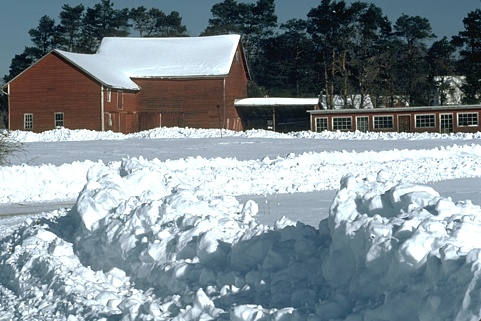
\includegraphics[width=0.3\columnwidth]{images/97033.jpg}  
}     
\subfigure[label 1] { \label{fig:b}     
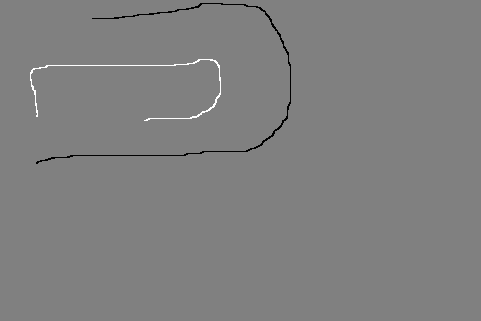
\includegraphics[width=0.3\columnwidth]{images/97033-5.png}     
}   
\subfigure[label 2] { \label{fig:b}     
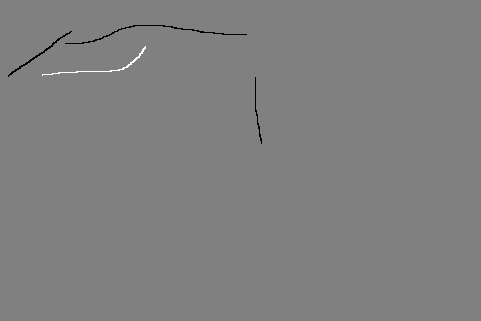
\includegraphics[width=0.3\columnwidth]{images/97033-4.png}     
}     
\caption{Two labels of the same image}     
\label{fig:example}     
\end{figure}


\subsection{Segmentation differences}
\paragraph{}Based on the above result, we took a step further by examine the segmentation results of different markers.The implementation of four interactive segmentation algorithms in \citep{gulshan2010geodesic} was used. Based on the 96*5*4 segmentation results, we have found out that due to the variance between different markers, the segmentation results tend to be quite different, too.  We achieved here by calculating percent of pixels which was segmented out as foreground simultaneously by 1 person, two people, three people ,four people and 5 people out of all the segmented pixels. The result is shown in Table 4-7. We have observed that: (1) The effectiveness of different markers as input of interactive segmentation algorithms vary from person to person.  It could also be observed that the seed made by participant 1 have a better performance than others in terms of average, maximum and minimum, which means there exists kind of "professional lables" \citep{fu2008saliency} (2) On average level, the result reaches at most 66.760\% in table 5 made by participant 1. While the maximum ratio could be high as 99.050\%, the minimum ratio was also low as 1.060\%. This shows that when applied to segmentation algorithms, the variance of markers could further lead to quite great difference in segmentation results. 


\begin{table}
\centering
\begin{tabular}{|c|c|}
\hline
Algorithm & Description\\
\hline
BJ &  Boykov Jolly Graph cut  \\
\hline
GSC & Boykov Jolly with Geodesic Star-Convexity \\
\hline
SP & Bai and Sapiro \\
\hline
RW & Random Walker  \\
\hline
\end{tabular}
\caption{intersection degree of background}
\end{table} 


\begin{table}
\centering
\begin{tabular}{|c|c|c|c|c|c|}
\hline
 intersection scale & 1 & 2 & 3 & 4& 5 \\
\hline
average& 66.360\% & 55.090\% & 52.300\% & 50.710\%& 49.620\% \\
\hline
max& 99.020\% & 98.580\% & 98.370\% & 98.200\%& 98.060\% \\
\hline
min& 21.060\% & 1.240\% & 1.180\% & 1.160\%& 1.140\%\\
\hline
variance& 0.0557 & 0.0883 & 0.0897 & 0.0899& 0.0898 \\
\hline
coefficient of variance& 0.3556 & 0.5394 & 0.5727 & 0.5913& 0.6039\\
\hline
\end{tabular}
\caption{bj}
\end{table} 

\begin{table}
\centering
\begin{tabular}{|c|c|c|c|c|c|}
\hline
intersection scale & 1 & 2 & 3 & 4& 5 \\
\hline
average& 66.760\% & 55.490\% & 52.490\% & 50.600\%& 49.170\% \\
\hline
max& 99.040\% & 98.500\% & 98.170\% & 97.900\%& 97.660\% \\
\hline
min& 21.130\% & 1.230\% & 1.100\% & 1.080\%& 1.060\%\\
\hline
variance& 0.0518 & 0.0809 & 0.0813 & 0.0812& 0.0812 \\
\hline
coefficient of variance& 0.3409 & 0.5126 & 0.5432 & 0.5632& 0.5795\\
\hline
\end{tabular}
\caption{gsc}
\end{table} 


\begin{table}
\centering
\begin{tabular}{|c|c|c|c|c|c|}
\hline
intersection scale & 1 & 2 & 3 & 4& 5 \\
\hline
average& 56.390\% & 41.030\% & 36.740\% & 34.350\%& 32.660\% \\
\hline
max& 96.040\% & 94.290\% & 93.470\% & 92.850\%& 92.260\% \\
\hline
min& 22.950\% & 2.920\% & 2.270\% & 2.030\%& 1.910\%\\
\hline
variance& 0.0286 & 0.0431 & 0.0418& 0.0405&0.0393 \\
\hline
coefficient of variance& 0.2999 & 0.5060 & 0.5565 & 0.5859& 0.6070\\
\hline
\end{tabular}
\caption{sp}
\end{table} 

\begin{table}
\centering
\begin{tabular}{|c|c|c|c|c|c|}
\hline
intersection scale & 1 & 2 & 3 & 4& 5 \\
\hline
average& 63.180\% & 49.860\% & 45.720\% & 43.180\%& 41.410\% \\
\hline
max& 98.660\% & 97.910\% & 97.430\% & 97.010\%& 96.600\% \\
\hline
min& 23.010\% & 3.190\% & 2.580\% & 2.190\%& 2.000\%\\
\hline
variance& 0.0295 & 0.0440 & 0.0432 & 0.0433& 0.0436 \\
\hline
coefficient of variance& 0.2719 & 0.4207 & 0.4546 & 0.4819& 0.5042\\
\hline
\end{tabular}
\caption{rw}
\end{table} 



\section{Automatic user interaction simulation}
\subsection{Quantitative of images}
\paragraph{} In interactive image segmentation,users are expected labels some key features of the image foreground and background. The effectiveness of these labels is greatly related to their coverage of foreground and background key components. So we decide to simulate markers by simulating their coverage of key pixel clusters. In our method, we used the simple linear iterative clustering (SLIC)  method \citep{achanta2010slic} implemented by VLFeat open source library\citep{vedaldi08vlfeat}. The SLIC algorithm clusters pixels in the combined five-dimensional color and image plane space which brings compact, nearly uniform superpixels. We then decompose all the superpixels into groups according to the quantitative feature of each superpixel. In this way, we could analyze user markers in superpixel level and superpixel group level.

\subsection{Quantitative simulation of user labels}
\paragraph{} Instead of continuous user scribbles, our simulation is targeted at generating several points to represent key features in the image. So our first step was to validate the effectiveness of points in segmentation as compared to continuous lines. After figuring out the superpixel groups which were covered by user markers, we randomly select one superpixel from these groups and then randomly select one point from that superpixel, in this way, we formed a point set which contains points from all groups covered by a certain artificial marker. We then applied five sets which were generated the same way to segmentation algorithms. In terms of evaluation of segmentation accuracy, we define the following criteria:
\begin{empheq}[box=\fbox]{align}
\begin{split}
 F_{gt} &= \text{foreground in ground truth}     \\
 F_{s}  &= \text{foreground in segmentation}     \\
  \text{recall}    &= \frac{F_{gt} \cap F_s}{F_{gt}}  \\
  \text{precision} &= \frac{F_{gt} \cap F_s}{F_{gt}}  \\
  \end{split}
\end{empheq}
The accuracy evaluation of five batches of markers and five batches of auto-generated seeds applied to the four algorithms are shown in the following tables(To be done).


\begin{table}
\centering
\begin{tabular}{|c|c|c|c|c|c|}
\hline
 & seed 1 & seed 2&seed 3&seed 4&seed 5 \\
\hline
Precision& 0.8595 & 0.8423 & 0.8449& 0.8543& 0.7474 \\
\hline
Recall& 0.8822 & 0.9158 & 0.9154& 0.9303& 0.9108 \\
\hline
 & simu-seed 1 & simu-seed 2&simu-seed 3&simu-seed 4&simu-seed 5 \\
 \hline
Precision& 63.180\% & 49.860\% & 45.720\%& 45.720\%& 45.720\% \\
\hline
Recall& 98.660\% & 97.910\% & 97.430\%& 45.720\%& 45.720\%  \\
\hline
\end{tabular}
\caption{bj}
\end{table} 

\begin{table}
\centering
\begin{tabular}{|c|c|c|c|c|c|}
\hline
 & seed 1 & seed 2&seed 3&seed 4&seed 5 \\
\hline
Precision& 0.8595 & 0.8423 & 0.8449& 0.8543& 0.7474 \\
\hline
Recall& 0.8822 & 0.9158 & 0.9154& 0.9303& 0.9108 \\
\hline
 & simu-seed 1 & simu-seed 2&simu-seed 3&simu-seed 4&simu-seed 5 \\
 \hline
Precision& 63.180\% & 49.860\% & 45.720\%& 45.720\%& 45.720\% \\
\hline
Recall& 98.660\% & 97.910\% & 97.430\%& 45.720\%& 45.720\%  \\
\hline
\end{tabular}
\caption{bj}
\end{table} 


\begin{table}
\centering
\begin{tabular}{|c|c|c|c|c|c|}
\hline
 & seed 1 & seed 2&seed 3&seed 4&seed 5 \\
\hline
Precision& 0.8595 & 0.8423 & 0.8449& 0.8543& 0.7474 \\
\hline
Recall& 0.8822 & 0.9158 & 0.9154& 0.9303& 0.9108 \\
\hline
 & simu-seed 1 & simu-seed 2&simu-seed 3&simu-seed 4&simu-seed 5 \\
 \hline
Precision& 63.180\% & 49.860\% & 45.720\%& 45.720\%& 45.720\% \\
\hline
Recall& 98.660\% & 97.910\% & 97.430\%& 45.720\%& 45.720\%  \\
\hline
\end{tabular}
\caption{bj}
\end{table} 


\begin{table}
\centering
\begin{tabular}{|c|c|c|c|c|c|}
\hline
 & seed 1 & seed 2&seed 3&seed 4&seed 5 \\
\hline
Precision& 0.8595 & 0.8423 & 0.8449& 0.8543& 0.7474 \\
\hline
Recall& 0.8822 & 0.9158 & 0.9154& 0.9303& 0.9108 \\
\hline
 & simu-seed 1 & simu-seed 2&simu-seed 3&simu-seed 4&simu-seed 5 \\
 \hline
Precision& 63.180\% & 49.860\% & 45.720\%& 45.720\%& 45.720\% \\
\hline
Recall& 98.660\% & 97.910\% & 97.430\%& 45.720\%& 45.720\%  \\
\hline
\end{tabular}
\caption{bj}
\end{table} 


\section{}









\begin{table}
\centering
\begin{tabular}{|c|c|c|c|}
\hline
& all-group-seed-1&all-group-seed-2&all-group-seed-3 \\
\hline
Precision&63.180\% &49.860\% &45.720\% \\
\hline
Recall&98.660\% &97.910\% &97.430\%  \\
\hline
\end{tabular}
\caption{rw}
\end{table} 






\bibliographystyle{plain}
\bibliography{references}

%\end{thebibliography}



\end{document}
